\section{Introduction}

Graph databases have become an important technology for managing highly connected data, with applications in social networks, knowledge graphs, recommendation systems, and biological networks \cite{angles2017foundations,bonifati2018querying}. Unlike relational systems, graph databases treat relationships as first-class elements, which makes them suited for queries that require navigation through connected data.

Modern graph query languages such as Cypher, SPARQL, SQL/PGQ, and GQL provide support for path-oriented queries \cite{angles2017foundations}. Such queries allow users to express reachability, pattern matching, and recursive navigation over graph structures. This makes path queries an important part of graph query languages and raises the question of how such operations can be described in a common algebraic framework.


For example, consider finding all paths between two nodes whose sequence of edge labels consists of one or more \texttt{KNOWS} relationships followed by zero or more \texttt{LIKES} relationships. Such path patterns can be described using regular expressions over edge labels and are common in graph query languages. Classical relational algebra does in contrast not provide a direct operator for recursive path traversal or transitive closure.

To illustrate, consider the following graph:

\begin{figure}[h!]
  \centering
  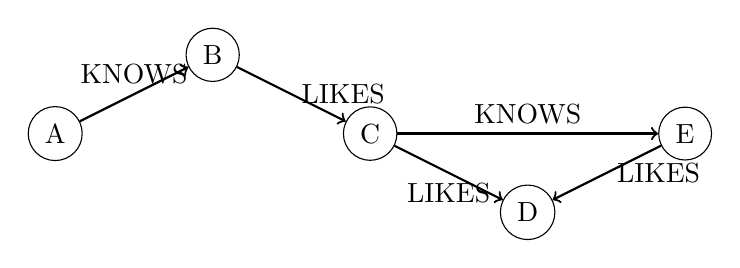
\begin{tikzpicture}
    % Nodes
    \node[circle, draw] (A) at (0,0) {A};
    \node[circle, draw] (B) at (2,1) {B};
    \node[circle, draw] (C) at (4,0) {C};
    \node[circle, draw] (D) at (6,-1) {D};
    \node[circle, draw] (E) at (8,0) {E};

    % Edges
    \draw[->, thick] (A) -- node[midway, above] {KNOWS} (B);
    \draw[->, thick] (B) -- node[midway, right] {LIKES} (C);
    \draw[->, thick] (C) -- node[midway, below] {LIKES} (D);
    \draw[->, thick] (C) -- node[midway, above] {KNOWS} (E);
    \draw[->, thick] (E) -- node[midway, right] {LIKES} (D);
  \end{tikzpicture}
  \caption{Example graph illustrating a path query.}
\end{figure}

In this graph, we seek all paths from node \texttt{A} to node \texttt{D} whose edge-label sequence matches the regular expression

\[
\texttt{KNOWS}^{+}\texttt{LIKES}^{*}.
\]

\[
A \xrightarrow{\texttt{KNOWS}} B
\xrightarrow{\texttt{LIKES}} C
\xrightarrow{\texttt{LIKES}} D
\]

This first path matches the pattern: it contains one \texttt{KNOWS} edge followed by two \texttt{LIKES} edges.

\[
A \xrightarrow{\texttt{KNOWS}} B
\xrightarrow{\texttt{LIKES}} C
\xrightarrow{\texttt{KNOWS}} E
\xrightarrow{\texttt{LIKES}} D
\]

This second path does not match because it contains a \texttt{KNOWS} edge after a \texttt{LIKES} edge.

In graph query languages, such patterns can be expressed using regular path expressions. For example, in GQL-inspired notation one could write:

\begin{Verbatim}
MATCH p = (A)-/:KNOWS+ LIKES*/->(D)
\end{Verbatim}

The essential idea is that the path must match the regular expression \texttt{KNOWS\textsuperscript{+}LIKES\textsuperscript{*}}. The example illustrates why path queries require operations for concatenation and recursion that are not part of classical relational algebra.
Relational algebra provides a foundation for relational query processing and optimization. For graph queries, however, an algebraic foundation for path-based operations is less established, especially when paths themselves are treated as query results.
Angles et al. propose a path algebra in which paths are treated as first-class data objects \cite{angles2024path}. It provides operators for path selection, concatenation, union, and recursion, and is intended to provide an algebraic basis for path queries in graph query languages such as GQL and SQL/PGQ.
This paper examines the core operators of the proposed path algebra and explains how they can be used to represent path queries. It then considers its relationship to relational algebra, automata-based approaches to regular path queries, and semiring-based models for graph problems.